\documentclass[a4paper,10pt]{article}
\usepackage{graphicx}
\usepackage{float}

% Title Page
\title{Assignment 1: Vacuum-Cleaning Agents}
\author{Francis Vo, Ryan Skeele}


\begin{document}
\maketitle
\begin{abstract}
Our goal was to study to performance of different types of agents; memory-less deterministic reflex agent, random reflex agent, and memory-based deterministic reflex agent.
We will measure the performance based on number of cleaned cells vs the number of actions taken.
The environment is a n X m empty rectangular room with p\% chance of containing dirt.
The agents have 5 actions; go forward, turn right by 90 degrees, turn left by 90 degrees, suck up dirt, and turn off.
The agents also have 3 sensor to interact with the room; a wall sensor, a dirt sensor, and a home sensor.
The memory-less agent, showed slightly higher efficiency than the memory-based agent.
The memory-based agent showed better performance and was gauranteed to clean the room, while the memory-less and random agents never cleaned more than 50 percent of the dirty tiles.
\end{abstract}

\section{Introduction}

In this paper we present our results for the generic vacuum cleaner world problem.
This problem has been used as a standard conceptual problem of AI for many years.
The vacuum cleaner world is a discretized environment that is n X m in dimension.
Each cell in this world has some percent (p) of containing dirt.
The goal of the vacuum cleaner is to find the cells containing dirt and clean them.
For this implementation of the vacuum problem we use one agent per experiment.
This agent doesn't know the state of the entire world, but can only observe based on three sensors; a front facing wall sensor, a dirt sensor, and a home sensor.
This means that the environment is partially observable.
In addition the sensors are modeled without uncertainty, making it a deterministic problem.
Lastly, the first two experiments are episodic because the agent experiences a precept and then performs a single action and that action does not depend on previous actions.
In the case of the third experiment the agent does make decisions based on previous actions, and the experiment is therefore sequential.

%Environment, partially observable, deterministic, single agent, sequential, discrete, known.
%Agents-overview. Memory restrictions

\section{Problem Formulation}
We run three experiments and compare the results.
Each experiment is in an environment of 10 x 10, or 100 cells.
The probability of dirt in each cell is varied from 0 to 100.
The five actions that can be taken are move forward, rotate 90 degrees left, rotate 90 degrees right, clean the current cell, and turn off.
The agent starts in the bottom left corner of the environment each time, this is defined as the agents home.
The experiment ends when the agent returns to the home position.
Each experiment is of a different agent in the same environment.
The three different agents are defined in the following sections.

\section{Agents}
Three different agents are used, a memory-less deterministic reflex agent, a random reflex agent, and a memory-based deterministic reflex agent.
In the following sections, for each agent the design and rules are explained followed by a discussion of the agents performance.
%Describe the idea behind the design of each of your agents. Use diagrams and English as appropriate.
\subsection{Memory-less Deterministic Reflex Agent}
\subsubsection{Design}
\begin{figure}[H]
	\begin{center}
		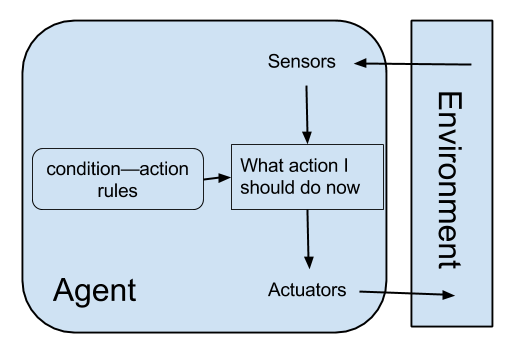
\includegraphics[width=0.6\textwidth]{MemorylessReflex.png}
	\end{center}
	% \caption{}
\end{figure}

The design for the memory-less deterministic reflex agent first uses its sensors to learn about its current location. Using that information, it follows condition-action rules to decide what to do next. The condition-action rules were designed to make the agent follow the wall around the room.

\subsubsection{If-then Rules}
\begin{verbatim}
if dirt then suck
else if wall then turn-right
else forward
\end{verbatim}

\subsubsection{Discussion}
%What is the best possible performance achievable by any memory-less reflex agent in this domain? What prevents a memory-less reflex agent from doing very well in this task?

Since the agent follows the wall around the room, it will always run over 36 cells.
So this means that it can only clean a maximum of 36 cells.
It takes 37 forward actions to travel the room, not including 3 turn actions, then takes one action to turn off.
This agent will always take 41 movement actions and a number of suck actions for the number of cells that were dirty on the side of the room.
Therefore we can conclude the performance is:

\[\frac{\mbox{number of cleaned cells}}{\mbox{41 movement actions} + \mbox{number of cleaned cells}}\]




\subsection{Random Reflex Agent}
%How well does the random agent perform? Do you think that this is the best possible performance achievable by any random agent? Why or why not? Give a table showing the number of actions it took to clean 90\% of the room for each trial. What is the average of these numbers for the best 45 trials? What are the costs and benefits of randomness in agent design?
\subsubsection{Design}
\begin{figure}[H]
	\begin{center}
		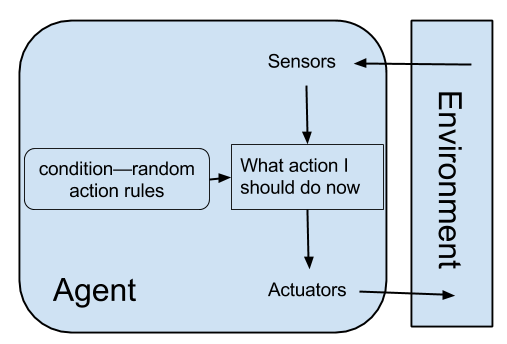
\includegraphics[width=0.6\textwidth]{RandomReflex.png}
	\end{center}
	% \caption{}
\end{figure}
\subsubsection{If-then Rules}
\begin{verbatim}
if dirt then suck
else if wall then turn-right 0.5 turn-left 0.5
else forward 0.5 turn-right 0.25 turn-left 0.25
\end{verbatim}


\subsection{Memory-Based Deterministic Reflex Agent}
\subsubsection{Design}
\begin{figure}[H]
	\begin{center}
		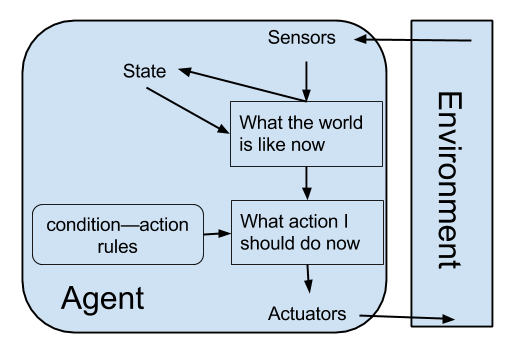
\includegraphics[width=0.6\textwidth]{MemoryReflex.png}
	\end{center}
	% \caption{}
\end{figure}

The memory-based deterministic reflex agent is similar to memory-less deterministic reflex agent, but it has more information about the world and its location with its 3-bit memory. 
This 3-bit memory allows the agent to know which direction its facing and if it took a turn recently.
In state 0, the agent knows that it is heading up.
In state 1, it just hit the north wall, and it is now facing right.
In state 2, it just turned after hitting the north wall, and it is facing right.
In state 3, it is now facing down. 
In state 4, it just hit the south wall, and it is now facing right.
In state 5, it just turned after hitting the south wall, and it is facing right.
In state 6, it just hit the east wall, now facing down, and on its way home.
In state 7, it just hit the south wall, now facing left, and on its way home.

Like the memory-less deterministic reflex agent, the performance could be calculated.
The agent will take 100 actions to move onto all the cells, 9 actions to visited cells on the way home, 20 turn actions, and 1 action to turn off. 
This agent will always take 130 movement actions and a number of suck actions for the number of cells that were dirty in the room. 
Therefore we can conclude the performance efficiency is:

\[\frac{\mbox{number of dirty cells}}{\mbox{130 movement actions} + \mbox{number of dirty cells}}\] 

\subsubsection{If-then Rules}
\begin{verbatim}
if dirt then suck
else if state0 and wall then turn-right set-state1
else if state1 and wall then turn-right set-state6
else if state1 and not wall then forward set-state2
else if state2 then turn-right set-state 3
else if state3 and wall then turn-left set-state4
else if state4 and wall then turn-right set-state6
else if state4 and not wall then forward set-state5
else if state5 then turn-left state-state0
else if state6 and wall then turn-right set-state7
else if state7 and home then off
else forward
\end{verbatim}

\subsubsection{Discussion}
%How does the memory-based deterministic agent perform compared to the random agent? Was it able to completely clean the room? Was it able to shut itself off after it is done? If it did, how many actions did it take to do this? Can the agent be improved any further with more memory than you used? Why or why not?

The memory-based deterministic agent took around the same number of actions compared to the random agent, but memory-based deterministic agent always left the room 100\% cleaned.
At the end of the random agent's run, 24\% to 100\% of the room was clean.
The efficiency was much higher than the random agent, the random agent took moves that went over visited cell and therefore wasted actions.
The memory-based deterministic agent also wasted actions finding its way home, but not as much as the random one.
The memory-based deterministic agent will completely clean the room, but it will take him 130 actions to clean a completely clean room.
With even more memory, the agent could map out the size of the room.
With the room size, it could create a better route without running over visited cells.
Also with the room size stored, it can save that knowledge for the next time it cleans the room, allowing for a better mapped route.


\section{Results}
Plots, discuss plots.

Plot 1- \%final dirt vs \% starting dirt \\
\begin{figure}[H]
	\begin{center}
		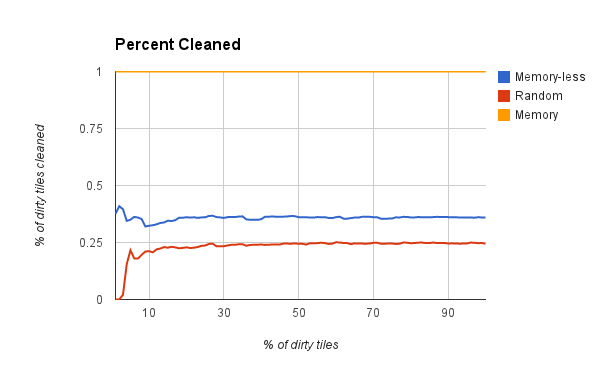
\includegraphics[width=0.9\textwidth]{image.png}
	\end{center}
	% \caption{}
\end{figure}
This graph measures the utility of each agent.
The utility is the usefulness of the agent to the user. 
The memory-based reflex agent always cleans 100\% of the dirt and therefore is very useful for the user.
The memoryless agent only cleans up to 36\% of the dirt because it only cleans the outer perimeter of the room.
The random agent cleaned a random 24\% of the dirt in the room. 

Plot 2- dirt per action vs \% starting dirt
\begin{figure}[H]
	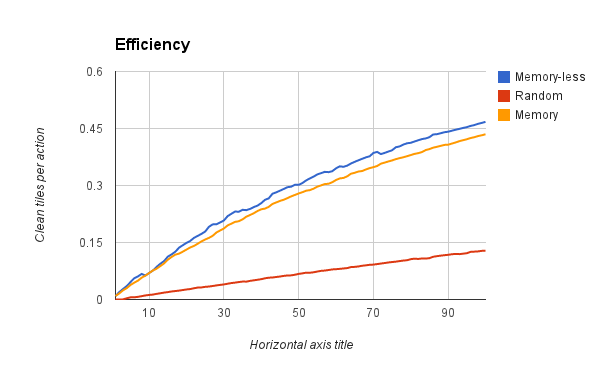
\includegraphics[width=0.9\textwidth]{image1.png}
\end{figure}

This graph shows the efficiency of each agent.

Plot 3- \# clean cells vs \# actions taken
\begin{figure}[H]
	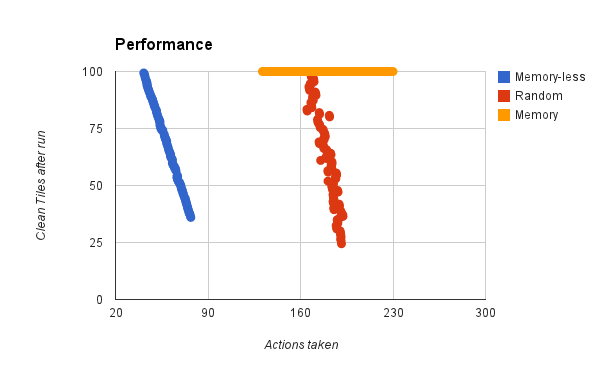
\includegraphics[width=0.9\textwidth]{image2.png}
\end{figure}

\section{Conclusion}
The experimental results are an interesting comparison of three agents with varying degrees of complexity.
We were surprised that the efficiency of the memory-less agent was higher than that of the more complex agents.
While the agent with memory was guaranteed to clean the entire environment, it was actually less efficient than the memoryless agent.
Similarly surprising was that the memory-less agent had a higher percentage cleaned than the random agent.
If it is more important that the whole area is cleaned then the Memory-based agent is gauranteed to perform the best.
If efficiency is more important (maybe due to battery restrictions on a robot) then the memory-based and memory-less are comparable, with the memory-less performing slightly better.
If the agent can only perform a small number of actions, the memory-less agent is the only option.
If the number of actions is not a limitation then the memory-based agent performs significantly better than the random agent in all metrics.
Our results show the benefits of each agent, and we learned that in not all metrics is a more complex agent better.
While this is a simple toy problem, what we learned may be extrapolated out to more complex real world situations.
Not always will the more complicated algorithm perform better.

Future work may include investigating agents with larger memory capabilities.
Additionally, it would be interesting to learn if adding more sensing capabilities to the agents would deliver different results.
Further simulations varying the size of the environment should also be explored.

%What did you learn from this experiment? Were you surprised by anything?
\end{document}
